\documentclass[11pt,a4paper]{amsart}
\usepackage[a4paper,margin=20mm]{geometry}
\usepackage{amsmath,amssymb,amsthm,mathtools,graphicx,xcolor,fontspec}
\usepackage{xspace,soul,microtype,multicol,paralist,tikz,comment}
\usetikzlibrary{automata,arrows.meta,tikzmark,calc,backgrounds}
\usepackage{hyperref}
\usepackage[capitalise]{cleveref}
\newtheorem{theorem}{Theorem}
\newtheorem{lemma}[theorem]{Lemma}
\newtheorem{corollary}[theorem]{Corollary}
\newtheorem{proposition}[theorem]{Proposition}
\theoremstyle{definition}
\newtheorem{definition}[theorem]{Definition}
\newtheorem{example}[theorem]{Example}
\newtheorem{remark}[theorem]{Remark}
\newtheorem{claim}[theorem]{Claim}
\newtheorem{observation}[theorem]{Observation}
\newtheorem{conjecture}[theorem]{Conjecture}
\AtBeginDocument{\def\shorttitle{Two-way one-counter nets}}
\newcommand{\shtodo}[1]{\todo[color=cyan!25,size=\small]{SH: #1}}
\newcommand{\shcomm}[2]{\st{#1}\todo[color=cyan!25,size=\small]{#2}}

\newcommand{\aytodo}[1]{\todo[inline,color=red!25,size=\small]{AY: #1}}

\newcommand{\tup}[1]{\langle #1 \rangle}
\newcommand{\lmark}{\vdash}
\newcommand{\rmark}{\dashv}
\newcommand{\pref}{\prec}
\newcommand{\eff}{\mathrm{eff}}

\newcommand{\initstate}{q_{\mathrm{init}}}
\newcommand{\accstate}{q_{\mathrm{acc}}}

\newcommand{\trans}[3]{#1,#2,#3}
\renewcommand{\vec}[1]{\boldsymbol{#1}}
\newcommand{\adds}[1]{\leftarrow #1}
\newcommand{\vf}[1]{\texttt{#1}}

\newcommand{\bbN}{\mathbb{N}}
\newcommand{\bbZ}{\mathbb{Z}}
\newcommand{\cA}{\mathcal{A}}
\newcommand{\cB}{\mathcal{B}}
\newcommand{\cD}{\mathcal{D}}
\newcommand{\cV}{\mathcal{V}}
\newcommand{\cR}{\mathcal{R}}
\newcommand{\cN}{\mathcal{N}}
\newcommand{\cM}{\mathcal{M}}


\newcommand{\raiseTikz}[1]{\raisebox{-2pt}{#1}\xspace}
\newcommand{\tikztapeax}{
	\draw[line width=0.3pt]  (0,0) rectangle (33pt,2ex);
	\fill[gray!50!white] (13pt,0.03ex) rectangle (20pt,1.97ex);
	\draw (25pt,2ex) -- (25pt,0ex);
	\draw (8pt,2ex) -- (8pt,0ex);
}

\newcommand{\emptytape}{\raiseTikz{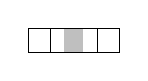
\begin{tikzpicture}
			\tikztapeax
		\end{tikzpicture}%
}}

%%% ALL THE DRAWINGS ARE UPDATED TO THE xa^Ky FORM
\newcommand{\leftloop}{\raiseTikz{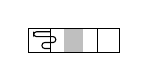
\begin{tikzpicture}
			\tikztapeax
			\draw [rounded corners=1pt] (8pt,1.7ex) -- (2pt,1.7ex) -- (2pt,1.3ex) -- (10pt,1.3ex) -- (10pt,.8ex) -- (5pt,.8ex) -- (5pt,0.3ex) -- (8pt,0.3ex);
		\end{tikzpicture}%
}}

\newcommand{\rightloop}{\raiseTikz{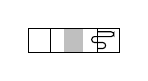
\begin{tikzpicture}
			\tikztapeax
			\draw [rounded corners=1pt] (25pt,1.7ex) -- (31pt,1.7ex) -- (31pt,1.3ex) -- (23pt,1.3ex) -- (23pt,.8ex) -- (28pt,.8ex) -- (28pt,0.3ex) -- (25pt,0.3ex);
		\end{tikzpicture}%
}}

\newcommand{\leftsink}{\raiseTikz{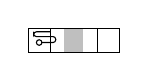
\begin{tikzpicture}
			\tikztapeax
			\draw [rounded corners=1pt] (8pt,1.7ex) -- (2pt,1.7ex) -- (2pt,1.3ex) -- (10pt,1.3ex) -- (10pt,.8ex) -- (5pt,.8ex);
			\draw (4pt,0.8ex) circle (1pt);
		\end{tikzpicture}%
}}

\newcommand{\rightsink}{\raiseTikz{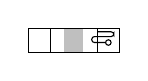
\begin{tikzpicture}
			\tikztapeax
			\draw [rounded corners=1pt] (25pt,1.7ex) -- (31pt,1.7ex) -- (31pt,1.3ex) -- (23pt,1.3ex) -- (23pt,.8ex) -- (28pt,.8ex);
			\draw (29pt,0.8ex) circle (1pt);
		\end{tikzpicture}%
}}

\newcommand{\rightcrossing}{\raiseTikz{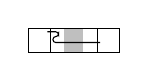
\begin{tikzpicture}
			\tikztapeax
			\draw [rounded corners=1pt] (7pt,1.7ex) -- (11pt,1.7ex) -- (11pt,1.3ex) -- (9pt,1.3ex) -- (9pt,.8ex) -- (26pt,.8ex);
		\end{tikzpicture}%
}}

\newcommand{\leftcrossing}{\raiseTikz{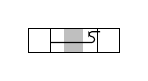
\begin{tikzpicture}
			\tikztapeax
			\draw [rounded corners=1pt] (26pt,1.7ex) -- (22pt,1.7ex) -- (22pt,1.3ex) -- (24pt,1.3ex) -- (24pt,.8ex) -- (8pt,.8ex);
		\end{tikzpicture}%
}}


\newcommand{\mysubparagraph}[1]{\noindent \textbf{\textsf{#1}} }
%\newcommand{\mysubpar}[1]{{\noindent \textsf{\textbf{#1}}}}

